This section is going to be about the possible design patterns, which is available to structure our system, implement a user interface, and eventually help simplify the testing process.

\subsubsection{MVC}

MVC stands for Model-View-Controller. The MVC pattern separates the application into three main components: Model, View and Controller. The model manages the behavior and data of the application, and responds to requests about its state, usually from the view through some kind of event, or the controller.  It also responds to instructions to change state, which is again issued by the view, but is performed through the controller. The view displays the state of the model through the graphical user interface, which as said, is received through the controllers, or indirectly by the model. \cite{Pattern1}

\subsubsection{MVVM}

Another pattern which which considered for this project was the MVVM pattern, which stands for Model View Viewmodel, its three main components. Like MVC, MVVM separates the system into three different components, creating a layered structure. The difference between is that MVVM is much more strict in this separation, which limits the model component to simply containing information about objects, and the view to simply provide a user interface. \cite{Pattern2}

The viewmodel is the component which implements most of the logical code, and is the binding point between the model and the view. The viewmodel implements commands, which for example is bound to a button on the view, together with restrictions, and take over the moment a user pushes said button. Beyond the button click, the view have given over full control to the viewmodel. The viewmodel also implements restrictions on the underlying model, so the properties and logic a model normally would have is located in the viewmodel instead. \cite{Pattern2}

\subsubsection{Comparison}

Both patterns provide this layered structure, which can help with testing the system later on, since it is divided into a workable bits following these patterns. For this project, the MVC pattern will be used, simply because it is the more simple of the two patterns, and still provides a good testing structure, despite being looser than the MVVM pattern. MVVM also requires more graphical design, since the view cannot have any notable code-behind. The technicalities behind graphical design is not the part of this projects goals, and is further reason for why MVC was chosen. The MVVM is also better suited for regular desk application, and since the one of the goals is the produce af web application, MVC was again weighed higher than MVVM.

\subsection{Implementation}

\begin{figure}[htb]
\centering
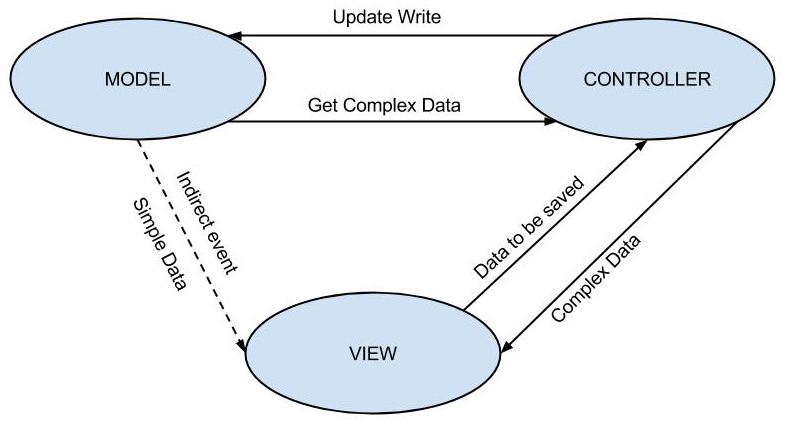
\includegraphics[width=1\textwidth]{Images/MVC.jpg}
\caption{How the MVC is planned to be implemented in this project}
\label{MVC}
\end{figure}

In the Figure \ref{MVC} above is a representation of how the MVC pattern is planned to be structured in our web application.

The model is the part of the MVC pattern which contains the general data of the systems classes, and their objects. You could say it is the database, or the class structure of the system. Besides storing class and object information, and communicating with other model members, the model component does not do much on its own, and is largely oblivious to the surrounding structure.

The controller is another part of the MVC pattern which gets information from the model and the view which does the “hard” work. It calculates depending on if it received information from the view or the model, and returns something to be shows on the view, or something to be stored in the model. It means the controller is the brain of the MVC pattern, and is the binding point between the view and the model.

The view is the part of the MVC pattern which basically is everything visually you can see and change on. What is viewed is usually the classes and objects which the model contains, which has been translated to a more understandable format in the graphical user interface, which the user then can see and manipulate. Any changes the user performs goes through the controller, and down into the model. The view is just as “stupid” as the model, as it cannot do much on its own, and depends on the controller, and indirect events.

The whole point of using the MVC pattern is to create some kind of layered system, dividing the responsibilities into several components. The MVC pattern can be done in various ways, for many different purposes, but this specific pattern is what we found the most appealing for this system. It places the largest need for testing onto the controllers, which contains most of the logical information processing, and the recommendation algorithm. While the graphical user interface is not completely interchangeable like it would be in a MVVM pattern, it is still easier to experiment and further develop with than without the MVC pattern.
